\documentclass[20pt]{beamer}
\usepackage[utf8]{inputenc}
\usepackage[T1]{fontenc}
\usepackage{lmodern}
\usepackage{graphicx}
\usetheme{default}
\usepackage{tabulary}


\newcommand\e{\emph}
\newcommand\tb{\textbf}
\newcommand\un{\underline}
\newcommand\txt{\texttt}


\begin{document}
	\author{Jennifer Lin}
	\title{Place of Residence and Political Attitudes in Democracies Worldwide}
	%\subtitle{}
	%\logo{}
	%\institute{New College of Florida}
	%\date{}
    %\subject{Transitions to Democracy}
	\setbeamercovered{transparent}
	\setbeamertemplate{navigation symbols}{}
	\begin{frame}[plain]
	\maketitle
\end{frame}

\begin{frame}
\frametitle{Research Question}
\begin{enumerate}
	\item Does place of residence influence political attitudes and ideology? 
	\item How do certain factors of the regime, including its age and electoral formula, influence these results?
\end{enumerate}
\end{frame}

\begin{frame}
\begin{itemize}
\frametitle{Literature}
\item Case specifications 
\item Analysis of Polities
\end{itemize}
\end{frame}

\begin{frame}
\frametitle{The United States}
\begin{figure}[H]    \centering
	{	 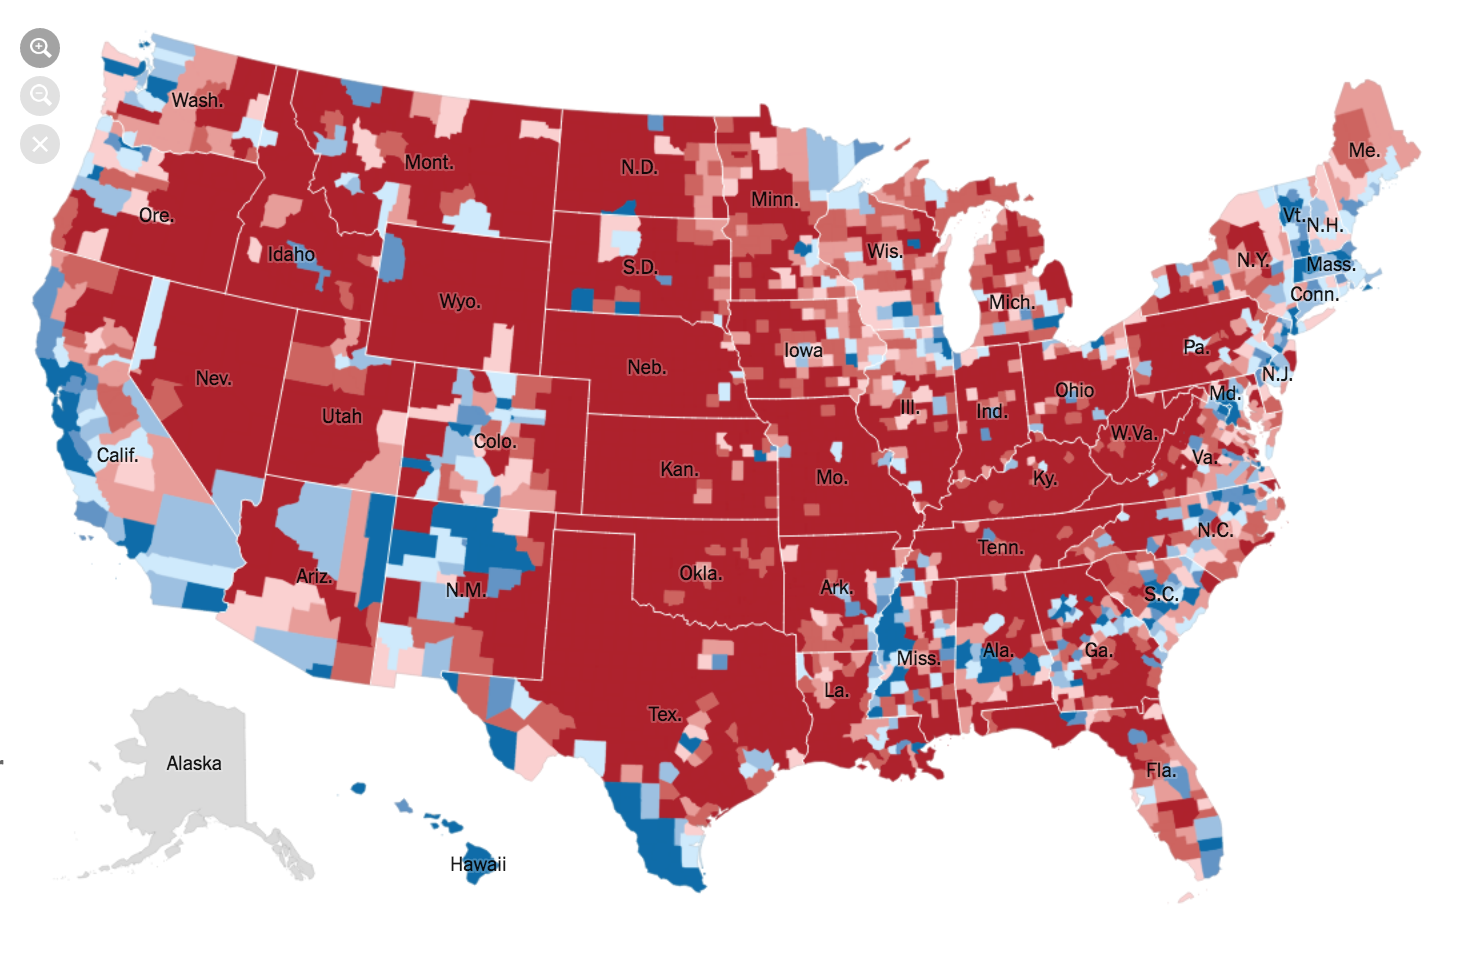
\includegraphics[width=\textwidth]{NYT}}
\end{figure}
\end{frame}

\begin{frame}
\frametitle{ALSO the United States}
\begin{figure}[H]    \centering
	{	 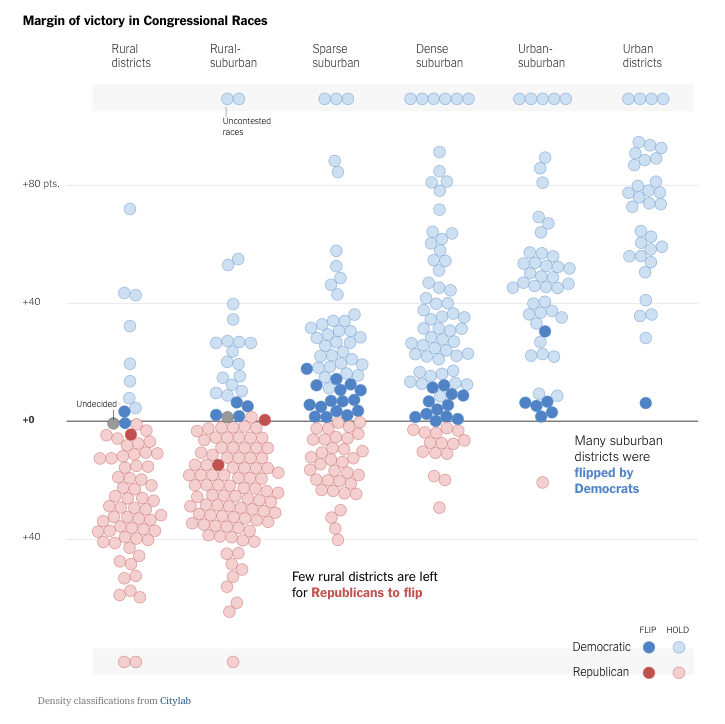
\includegraphics[width=.7\textwidth]{ClayLab}}
\end{figure}
\end{frame}

\begin{frame}
\frametitle{NOT the United States}
\begin{figure}[H]    \centering
	{	 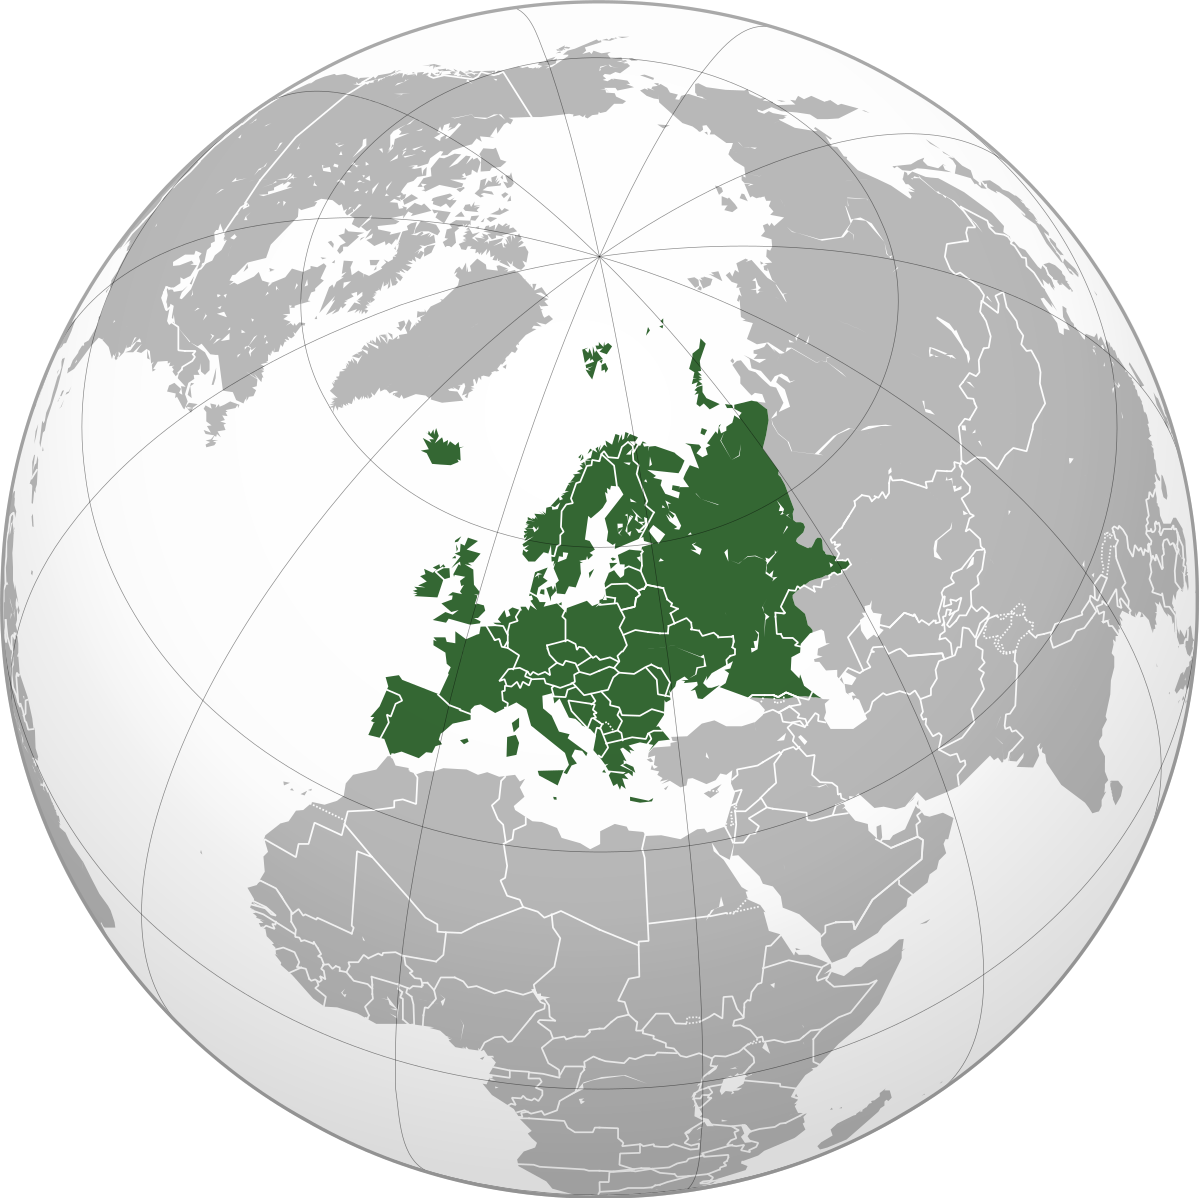
\includegraphics[width=.7\textwidth]{Europe}}
\end{figure}
\end{frame}

\begin{frame}
\frametitle{Polities in the CSES}
\begin{figure}[ht!]    \centering
	{	 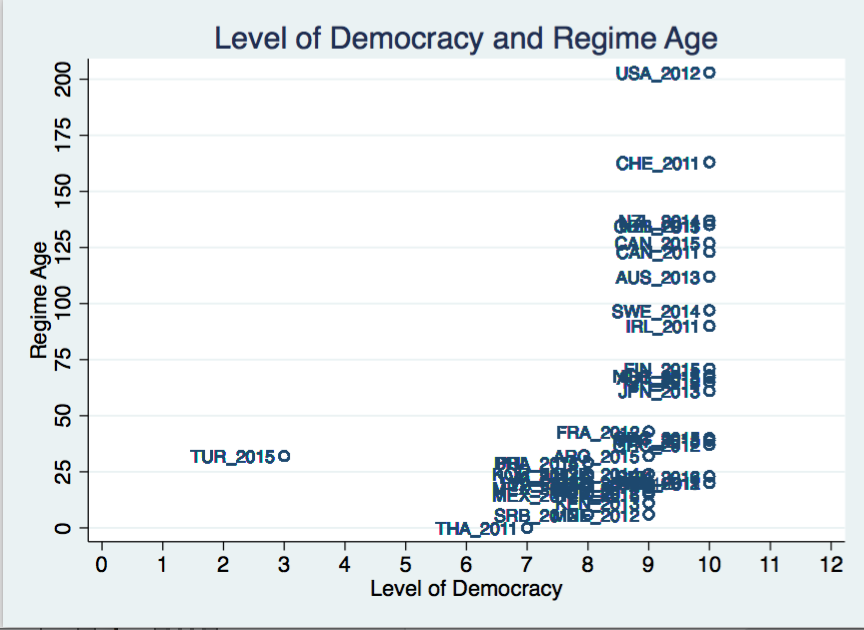
\includegraphics[width=.8\textwidth]{DemAge}}
\end{figure}
\end{frame}

\begingroup
\begin{frame}
\footnotesize
\frametitle{Hypotheses}
\e {Hypothesis 1 -- Place Matters} \\
~~\\
\e{Hypothesis 2 -- Issue Stances} \\
~~\\
\e{Hypothesis 3A -- Level of Democracy} \\
~~\\
\e{Hypothesis 3B -- Regime Age} \\
~~\\
\e{Hypothesis 3C -- Electoral Formula}\\
~~\\
\e{Hypothesis 3D -- Polity Differences} 

\end{frame}

\begin{frame}
\frametitle{Data - CSES Module IV}
\begin{figure}[H]    \centering
	{	 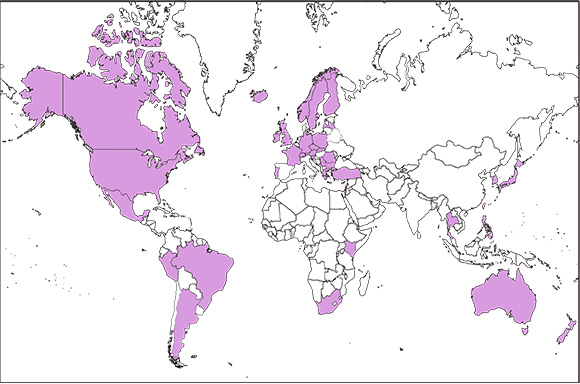
\includegraphics[width=.9\textwidth]{Mod4}}
\end{figure}
\end{frame}

\begin{frame}
\frametitle{Independent Measures}
\begin{itemize}
	\item Country
	\item Place of Residence
	\item Level of Democracy
	\item Regime Age
	\item Electoral Formula
\end{itemize}
\end{frame}

\begin{frame}

\frametitle{Dependent Measures}
\begin{itemize}
	\item Self-Placement Ideology (0-10)
	\item Liberalism - Public Expenditure and Income Inequality
\end{itemize}
\end{frame}

\begin{frame}
\tiny
%\frametitle{Results - Ideology and Liberalism}
\begin{table}[H]
	\centering
	\def\arraystretch{1}
	\caption{\tb{General Trends of Ideology}}
	\begin{tabulary}{\linewidth}{l c c}
		\hline
		\tb{Place of Residence}&\tb{Self-Placement} & \tb{Liberalism} \\
		\hline
		Small Town&-.1338***& -.1005*** \\    
		& (.0336) & (.0136)  \\
		Suburban & -.2591*** &-.1737 ***\\ 
		& (.0358) &(.0162) \\
		Urban   & -.0482 &-.1309***  \\
		& (.0300)  &(.123)  \\
		Constant   & 5.597*** &5.7164*** \\
		&(.0234) & (.0093)\\
		N  & 47,821 & 42,500 \\
		$R^2$	& 0.0011 & 0.0037 \\
		\hline                                       
	\end{tabulary}
	\\
	\e{Notes:} *p$<$.1, **p$<$.05. ***p$<$.01 \\
	\e{Reference:} A rural place of residence serves as the baseline for comparison
\end{table}
\end{frame}

\begin{frame}
\frametitle{Regional Urban-Rural Splits}
\begin{figure}[H]    \centering
	{	 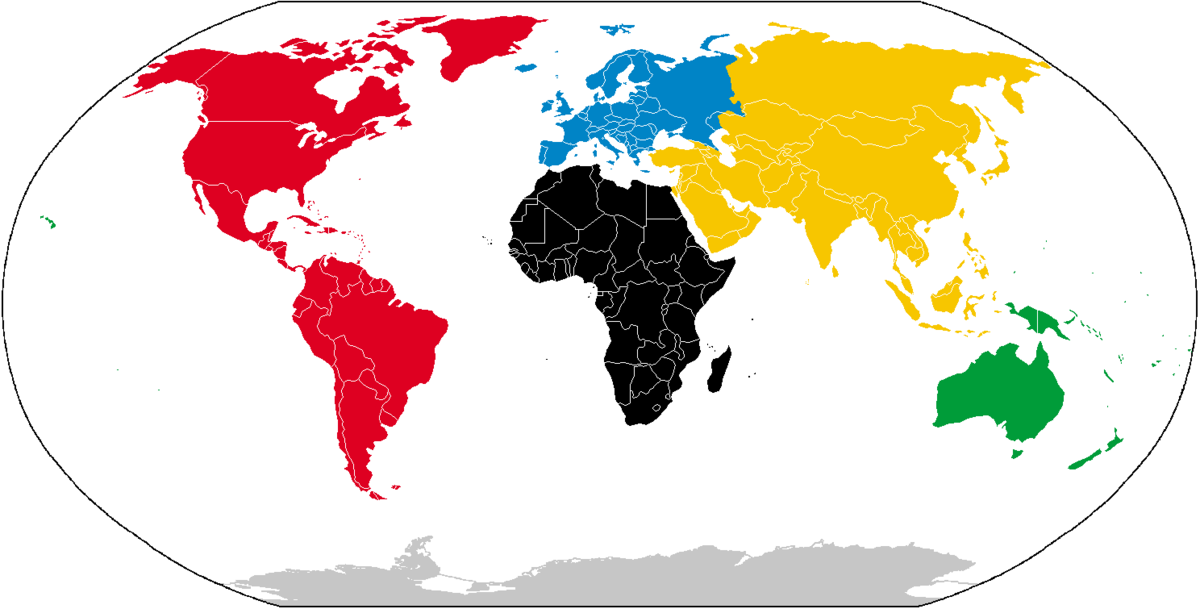
\includegraphics[width=\textwidth]{Regions}}
\end{figure}
\end{frame}

\begin{frame}
\frametitle{Macro Variables}
\begin{enumerate}
	\item Level of Democracy
	\item Regime Age
	\item Electoral Formula
\end{enumerate}	
\end{frame}

\begin{frame}
\tiny
\begin{table}[h!]
	\centering
	\caption{\tb{By Electoral Formula}}
	\begin{tabulary}{\linewidth}{l c c c}
		\\
		\hline
		\tb{Place of Residence}&\tb{Majoritarian}&\tb{Proportional} &\tb{Mixed} \\
		\hline
		Small Town&-.6640*** &.0608 &-.1600** \\
		&(.0766)&(.0435) &(.0727) \\
		Suburban&-.6389*** &-.1894***&-.1260  \\
		&(.1042) &(.0451) &(.1180) \\
		Urban&-.5781*** &-.0327 &.2655*** \\
		&(.0710) &(.0388) &(.0644) \\
		Constant& 5.8256*** &5.5408***&5.5562*** \\
		&(.0543) &(.0297) &(.0531) \\
		Countries&5&21&6 \\
		N&8,350&28,869 &10,602 \\
		$R^2$&0.0114&0.0011 &0.0052 \\
		\hline 
	\end{tabulary} 
	\\ 
	\e{Notes:} *p$<$.1, **p$<$.05. ***p$<$.01 \\
	\e{Reference:} A rural place of residence serves as the baseline for comparison
\end{table}
\end{frame}

\begin{frame}
\tiny
\begin{table}[h!]
	\centering
	%\def\arraystretch{1.5}
	\begin{tabulary}{\linewidth}{l c c}
		\hline
		\tb{Variable}&\tb{Self-Placement}&\tb{Liberalism} \\
		\hline
		\e{Place of Residence} & & \\
		Small Town &-.1000***&-.0018 \\
		&(.0339)&(.0130) \\
		Suburban& -.1517***& .0147 \\
		&(.0401)& (.0157) \\
		Urban&-.0517* & -.0420*** \\
		&(.0304) & (.0117) \\
		\e{Democracy}& -.1995*** & -.0421***\\
		&(.0110) & (.0040)\\
		\e{Regime Age} & -.0014*** &  -.0075***\\
		&(.0002) & (.0001)\\
		\e{Electoral Formula}&.0778*** & -.0440***\\
		&(.0189) & (.0070) \\
		\hline
		Constant& 7.3627*** & 6.5149*** \\
		&(.1067) & (.0391)\\
		N&46,555 & 41,373 \\
		$R^2$&0.0135& 0.1273 \\
		\hline
	\end{tabulary}
	\\
	\e{Notes:} *p$<$.1, **p$<$.05. ***p$<$.01 \\
	\e{Reference:} A rural place of residence serves as the baseline for comparison
\end{table}
\end{frame}

\begin{frame}
\footnotesize
\frametitle{Hypotheses Revisited}

\e {Hypothesis 1 -- Place Matters} \\
~~\\
\e{Hypothesis 2 -- Issue Stances} \\
~~\\
\e{Hypothesis 3A -- Level of Democracy} \\
~~\\
\e{Hypothesis 3B -- Regime Age} \\
~~\\
\e{Hypothesis 3C -- Electoral Formula}\\
~~\\
\e{Hypothesis 3D -- Polity Differences} 

\end{frame}

\begin{frame}
\frametitle{Conclusions}
\begin{figure}[H]    \centering
	{	 
\includegraphics[width=\textwidth]{RuralUrban}}
\end{figure}
\end{frame}
\endgroup

\begin{frame}
\frametitle{That's All, Folks!}
\begin{figure}[H]    \centering
	{	 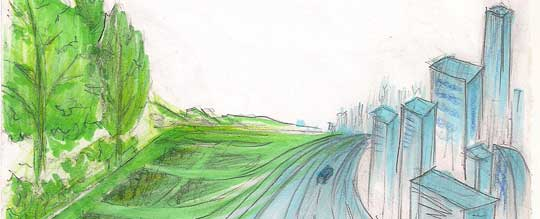
\includegraphics[width=\textwidth]{Sketch}}
\end{figure}
\end{frame}

\end{document}